\section{Results}

We implement our model (\autoref{fig:full-model}) using the \texttt{pytorch} python library \cite{pytorch}. Code and instructions for reproducing these results are available on GitHub \cite{stat-comps-github}. To train our model, we use the binary cross-entropy loss function where each output $p_t$ is compared to the true outcome of the game
\begin{equation}
	y = \begin{cases}
		1 & \text{if the home team wins}  \\
		0 & \text{if the away team wins}.
	\end{cases}
\end{equation}
We fit our models using gradient descent via backpropogation with respect to this loss function.

To measure our model's performance, we use what is known as \emph{cross-validation}, a model evaluation technique in which we measure model fitness based on how well it performs on data that was not used during the training phase.
More precisely, we split our data into two subsets known as the \emph{training} and \emph{validation} (or \emph{test}) subsets---typically one uses an 80-20 percent split. We fit our model only on the training subset and then measure its performance on the validation subset. If the training performance exceeds the validation performance by a significant margin, we say that our model has \emph{overfit}, i.e., learned patterns that are in the training data by chance and are not indicative of a real relationship.

The results of our model training are given in \autoref{tbl:model-results}. The training/validation curves (performance as a function of training time) for each model are shown in \autoref{fig:training-curves}.

\begin{table}
	\begin{tabular}{r l  ccccc}
		         &      &       & \multicolumn{2}{c}{\underline{Training}} & \multicolumn{2}{c}{\underline{Validation}}                     \\
		RNN type & Size & Epoch & Loss                                     & Accuracy                                   & Loss   & Accuracy \\
		\hline
		GRU      & xs   & 20    & 0.5046                                   & 0.7394                                     & 0.5112 & 0.7373   \\
		         & sm   & 16    & 0.4998                                   & 0.7383                                     & 0.5073 & 0.7385   \\
		         & md   & 17    & 0.4938                                   & 0.7400                                     & 0.5013 & 0.7378   \\
		         & lg   & 20    & 0.4880                                   & 0.7431                                     & 0.5013 & 0.7397   \\
		         & xl   & 10    & 0.5053                                   & 0.7378                                     & 0.5089 & 0.7381   \\
		\hline
		LSTM     & xs   & 14    & 0.5066                                   & 0.7410                                     & 0.5179 & 0.7363   \\
		         & sm   & 17    & 0.4995                                   & 0.7386                                     & 0.5052 & 0.7377   \\
		         & md   & 20    & 0.4914                                   & 0.7430                                     & 0.5006 & 0.7388   \\
		         & lg   & 15    & 0.4964                                   & 0.7406                                     & 0.5048 & 0.7378   \\
		         & xl   & 20    & 0.5034                                   & 0.7351                                     & 0.5035 & 0.7380   \\
		\hline
		Elman    & xs   & 16    & 0.5153                                   & 0.7382                                     & 0.5166 & 0.7382   \\
		         & sm   & 20    & 0.4973                                   & 0.7382                                     & 0.5000 & 0.7393   \\
		         & md   & 19    & 0.4942                                   & 0.7419                                     & 0.4970 & 0.7402   \\
		         & lg   & 12    & 0.4961                                   & 0.7415                                     & 0.5017 & 0.7395   \\
		         & xl   & 13    & 0.4984                                   & 0.7392                                     & 0.5109 & 0.7385   \\
		\hline
	\end{tabular}
	\caption{The performance of our various models, taken at the epoch (round of training) in which validation accuracy is maximized. Because there is no notion of a ``positive'' and ``negative'' label in our classification problem, we do not evaluate our models' precision.}
	\label{tbl:model-results}
\end{table}

At first, these results are quite encouraging: Every model achieves a validation accuracy of at least 73 percent, and the complex models do not seem to provide any meaningful boost in performance. However, the larger models do appear to converge more quickly (\autoref{fig:training-curves}). No model appears to suffer from overfitting.

However, the fanfare fades when we realize that the simple classifier that predicts the currently-ahead team to win has an accuracy of 73.143 percent. All of our models do slightly out-perform this, but without something like an $F$-statistic, it's difficult to say whether this is a meaningful improvement.
Examining the Shapley values\footnote{Shapley values are a game-theory based approach that adds random noise to samples in order to estimate the influence of each predictor on a model's outcome} \cite{captum, shap-paper} for the model with the best validation accuracy (Elman RNN, medium size) indicates that our complex neural networks have learned to focus almost entirely on each teams' score (\autoref{fig:model-shap-values}).
We discuss the implications and potential causes of this in the following section.

\begin{figure}
	\centering
	% Created by tikzDevice version 0.12.4 on 2024-02-26 09:01:11
% !TEX encoding = UTF-8 Unicode
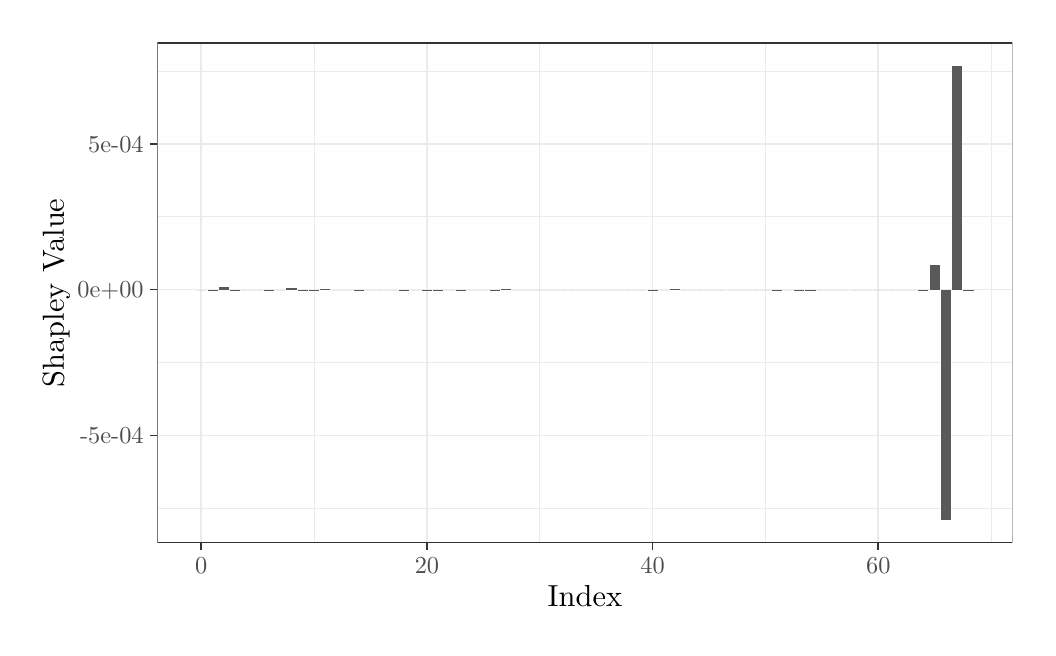
\begin{tikzpicture}[x=1pt,y=1pt]
\definecolor{fillColor}{RGB}{255,255,255}
\path[use as bounding box,fill=fillColor] (0,0) rectangle (361.35,216.81);
\begin{scope}
\path[clip] (  0.00,  0.00) rectangle (361.35,216.81);
\definecolor{drawColor}{RGB}{255,255,255}

\path[draw=drawColor,line width= 0.6pt,line join=round,line cap=round,fill=fillColor] (  0.00,  0.00) rectangle (361.35,216.81);
\end{scope}
\begin{scope}
\path[clip] ( 46.86, 30.69) rectangle (355.85,211.31);
\definecolor{fillColor}{RGB}{255,255,255}

\path[fill=fillColor] ( 46.86, 30.69) rectangle (355.85,211.31);
\definecolor{drawColor}{gray}{0.92}

\path[draw=drawColor,line width= 0.3pt,line join=round] ( 46.86, 43.16) --
	(355.85, 43.16);

\path[draw=drawColor,line width= 0.3pt,line join=round] ( 46.86, 95.83) --
	(355.85, 95.83);

\path[draw=drawColor,line width= 0.3pt,line join=round] ( 46.86,148.49) --
	(355.85,148.49);

\path[draw=drawColor,line width= 0.3pt,line join=round] ( 46.86,201.16) --
	(355.85,201.16);

\path[draw=drawColor,line width= 0.3pt,line join=round] (103.51, 30.69) --
	(103.51,211.31);

\path[draw=drawColor,line width= 0.3pt,line join=round] (185.05, 30.69) --
	(185.05,211.31);

\path[draw=drawColor,line width= 0.3pt,line join=round] (266.59, 30.69) --
	(266.59,211.31);

\path[draw=drawColor,line width= 0.3pt,line join=round] (348.12, 30.69) --
	(348.12,211.31);

\path[draw=drawColor,line width= 0.6pt,line join=round] ( 46.86, 69.49) --
	(355.85, 69.49);

\path[draw=drawColor,line width= 0.6pt,line join=round] ( 46.86,122.16) --
	(355.85,122.16);

\path[draw=drawColor,line width= 0.6pt,line join=round] ( 46.86,174.83) --
	(355.85,174.83);

\path[draw=drawColor,line width= 0.6pt,line join=round] ( 62.74, 30.69) --
	( 62.74,211.31);

\path[draw=drawColor,line width= 0.6pt,line join=round] (144.28, 30.69) --
	(144.28,211.31);

\path[draw=drawColor,line width= 0.6pt,line join=round] (225.82, 30.69) --
	(225.82,211.31);

\path[draw=drawColor,line width= 0.6pt,line join=round] (307.36, 30.69) --
	(307.36,211.31);
\definecolor{fillColor}{gray}{0.35}

\path[fill=fillColor] ( 60.91,122.16) rectangle ( 64.58,122.16);

\path[fill=fillColor] ( 64.99,121.96) rectangle ( 68.66,122.16);

\path[fill=fillColor] ( 69.06,122.16) rectangle ( 72.73,123.04);

\path[fill=fillColor] ( 73.14,121.81) rectangle ( 76.81,122.16);

\path[fill=fillColor] ( 77.22,122.16) rectangle ( 80.89,122.16);

\path[fill=fillColor] ( 81.29,122.16) rectangle ( 84.96,122.16);

\path[fill=fillColor] ( 85.37,121.56) rectangle ( 89.04,122.16);

\path[fill=fillColor] ( 89.45,122.16) rectangle ( 93.12,122.16);

\path[fill=fillColor] ( 93.52,122.16) rectangle ( 97.19,122.70);

\path[fill=fillColor] ( 97.60,122.16) rectangle (101.27,122.17);

\path[fill=fillColor] (101.68,121.98) rectangle (105.35,122.16);

\path[fill=fillColor] (105.75,122.16) rectangle (109.42,122.38);

\path[fill=fillColor] (109.83,122.16) rectangle (113.50,122.16);

\path[fill=fillColor] (113.91,122.16) rectangle (117.58,122.16);

\path[fill=fillColor] (117.99,122.15) rectangle (121.65,122.16);

\path[fill=fillColor] (122.06,122.16) rectangle (125.73,122.16);

\path[fill=fillColor] (126.14,122.16) rectangle (129.81,122.16);

\path[fill=fillColor] (130.22,122.16) rectangle (133.88,122.16);

\path[fill=fillColor] (134.29,122.16) rectangle (137.96,122.18);

\path[fill=fillColor] (138.37,122.16) rectangle (142.04,122.16);

\path[fill=fillColor] (142.45,122.12) rectangle (146.12,122.16);

\path[fill=fillColor] (146.52,122.14) rectangle (150.19,122.16);

\path[fill=fillColor] (150.60,122.16) rectangle (154.27,122.16);

\path[fill=fillColor] (154.68,122.12) rectangle (158.35,122.16);

\path[fill=fillColor] (158.75,122.16) rectangle (162.42,122.16);

\path[fill=fillColor] (162.83,122.16) rectangle (166.50,122.16);

\path[fill=fillColor] (166.91,122.02) rectangle (170.58,122.16);

\path[fill=fillColor] (170.98,122.16) rectangle (174.65,122.28);

\path[fill=fillColor] (175.06,122.16) rectangle (178.73,122.16);

\path[fill=fillColor] (179.14,122.16) rectangle (182.81,122.16);

\path[fill=fillColor] (183.22,122.16) rectangle (186.88,122.16);

\path[fill=fillColor] (187.29,122.16) rectangle (190.96,122.16);

\path[fill=fillColor] (191.37,122.16) rectangle (195.04,122.16);

\path[fill=fillColor] (195.45,122.16) rectangle (199.11,122.16);

\path[fill=fillColor] (199.52,122.16) rectangle (203.19,122.16);

\path[fill=fillColor] (203.60,122.16) rectangle (207.27,122.16);

\path[fill=fillColor] (207.68,122.16) rectangle (211.35,122.16);

\path[fill=fillColor] (211.75,122.16) rectangle (215.42,122.16);

\path[fill=fillColor] (215.83,122.16) rectangle (219.50,122.16);

\path[fill=fillColor] (219.91,122.16) rectangle (223.58,122.16);

\path[fill=fillColor] (223.98,122.11) rectangle (227.65,122.16);

\path[fill=fillColor] (228.06,122.16) rectangle (231.73,122.16);

\path[fill=fillColor] (232.14,122.16) rectangle (235.81,122.24);

\path[fill=fillColor] (236.21,122.16) rectangle (239.88,122.16);

\path[fill=fillColor] (240.29,122.16) rectangle (243.96,122.16);

\path[fill=fillColor] (244.37,122.16) rectangle (248.04,122.16);

\path[fill=fillColor] (248.44,122.16) rectangle (252.11,122.16);

\path[fill=fillColor] (252.52,122.16) rectangle (256.19,122.16);

\path[fill=fillColor] (256.60,122.16) rectangle (260.27,122.16);

\path[fill=fillColor] (260.68,122.16) rectangle (264.34,122.16);

\path[fill=fillColor] (264.75,122.16) rectangle (268.42,122.16);

\path[fill=fillColor] (268.83,122.08) rectangle (272.50,122.16);

\path[fill=fillColor] (272.91,122.16) rectangle (276.58,122.16);

\path[fill=fillColor] (276.98,122.16) rectangle (280.65,122.17);

\path[fill=fillColor] (281.06,122.16) rectangle (284.73,122.17);

\path[fill=fillColor] (285.14,122.16) rectangle (288.81,122.16);

\path[fill=fillColor] (289.21,122.16) rectangle (292.88,122.16);

\path[fill=fillColor] (293.29,122.16) rectangle (296.96,122.16);

\path[fill=fillColor] (297.37,122.16) rectangle (301.04,122.16);

\path[fill=fillColor] (301.44,122.16) rectangle (305.11,122.16);

\path[fill=fillColor] (305.52,122.16) rectangle (309.19,122.16);

\path[fill=fillColor] (309.60,122.16) rectangle (313.27,122.16);

\path[fill=fillColor] (313.67,122.16) rectangle (317.34,122.16);

\path[fill=fillColor] (317.75,122.16) rectangle (321.42,122.16);

\path[fill=fillColor] (321.83,122.03) rectangle (325.50,122.16);

\path[fill=fillColor] (325.91,122.16) rectangle (329.57,130.94);

\path[fill=fillColor] (329.98, 38.90) rectangle (333.65,122.16);

\path[fill=fillColor] (334.06,122.16) rectangle (337.73,203.10);

\path[fill=fillColor] (338.14,121.60) rectangle (341.81,122.16);
\definecolor{drawColor}{gray}{0.20}

\path[draw=drawColor,line width= 0.6pt,line join=round,line cap=round] ( 46.86, 30.69) rectangle (355.85,211.31);
\end{scope}
\begin{scope}
\path[clip] (  0.00,  0.00) rectangle (361.35,216.81);
\definecolor{drawColor}{gray}{0.30}

\node[text=drawColor,anchor=base east,inner sep=0pt, outer sep=0pt, scale=  0.88] at ( 41.91, 66.46) {-5e-04};

\node[text=drawColor,anchor=base east,inner sep=0pt, outer sep=0pt, scale=  0.88] at ( 41.91,119.13) {0e+00};

\node[text=drawColor,anchor=base east,inner sep=0pt, outer sep=0pt, scale=  0.88] at ( 41.91,171.80) {5e-04};
\end{scope}
\begin{scope}
\path[clip] (  0.00,  0.00) rectangle (361.35,216.81);
\definecolor{drawColor}{gray}{0.20}

\path[draw=drawColor,line width= 0.6pt,line join=round] ( 44.11, 69.49) --
	( 46.86, 69.49);

\path[draw=drawColor,line width= 0.6pt,line join=round] ( 44.11,122.16) --
	( 46.86,122.16);

\path[draw=drawColor,line width= 0.6pt,line join=round] ( 44.11,174.83) --
	( 46.86,174.83);
\end{scope}
\begin{scope}
\path[clip] (  0.00,  0.00) rectangle (361.35,216.81);
\definecolor{drawColor}{gray}{0.20}

\path[draw=drawColor,line width= 0.6pt,line join=round] ( 62.74, 27.94) --
	( 62.74, 30.69);

\path[draw=drawColor,line width= 0.6pt,line join=round] (144.28, 27.94) --
	(144.28, 30.69);

\path[draw=drawColor,line width= 0.6pt,line join=round] (225.82, 27.94) --
	(225.82, 30.69);

\path[draw=drawColor,line width= 0.6pt,line join=round] (307.36, 27.94) --
	(307.36, 30.69);
\end{scope}
\begin{scope}
\path[clip] (  0.00,  0.00) rectangle (361.35,216.81);
\definecolor{drawColor}{gray}{0.30}

\node[text=drawColor,anchor=base,inner sep=0pt, outer sep=0pt, scale=  0.88] at ( 62.74, 19.68) {0};

\node[text=drawColor,anchor=base,inner sep=0pt, outer sep=0pt, scale=  0.88] at (144.28, 19.68) {20};

\node[text=drawColor,anchor=base,inner sep=0pt, outer sep=0pt, scale=  0.88] at (225.82, 19.68) {40};

\node[text=drawColor,anchor=base,inner sep=0pt, outer sep=0pt, scale=  0.88] at (307.36, 19.68) {60};
\end{scope}
\begin{scope}
\path[clip] (  0.00,  0.00) rectangle (361.35,216.81);
\definecolor{drawColor}{RGB}{0,0,0}

\node[text=drawColor,anchor=base,inner sep=0pt, outer sep=0pt, scale=  1.10] at (201.36,  7.64) {Index};
\end{scope}
\begin{scope}
\path[clip] (  0.00,  0.00) rectangle (361.35,216.81);
\definecolor{drawColor}{RGB}{0,0,0}

\node[text=drawColor,rotate= 90.00,anchor=base,inner sep=0pt, outer sep=0pt, scale=  1.10] at ( 13.08,121.00) {Shapley Value};
\end{scope}
\end{tikzpicture}

	\caption{The Shapley values for our model, which roughly measure the contribution of each column in our data to our model's predictions. The two big peaks correspond to the columns encoding away team score (which has a large negative effect on the home team winning) and home team score (which has a large positive effect). This plot supports the notion that our model has simply learned to pick the team currently in the lead, although the smaller peak just to the left hints that our model is also doing something with the information about the time remaining.}
	\label{fig:model-shap-values}
\end{figure}

